\documentclass[10pt,conference,twocolumn]{IEEEtran}
\hyphenation{op-tical net-works semi-conduc-tor}
\usepackage{graphicx}
\usepackage{setspace}
\usepackage{makeidx}
\usepackage{mdframed}
\usepackage{amsmath}
\usepackage[ruled]{algorithm2e}
\renewcommand{\algorithmcfname}{ALGORITHM}
\usepackage{amsmath}
\usepackage{algpseudocode}
\usepackage[autostyle]{csquotes}
\usepackage{wrapfig}
\usepackage{float}
\usepackage{hyperref}
\usepackage{cite}
\makeindex
\title{\LARGE{Why-Diff: Exploiting Execution Provenance to Answer the Difference Between Two Computational Results}}
\author{Priyaa Thavasimani}
%\date{June 2016} %Insert leading % sign for today's date.
\usepackage{graphicx}
\usepackage{setspace}
\usepackage{makeidx}
\usepackage{mdframed}
\usepackage[autostyle]{csquotes}
\usepackage{caption}
\usepackage{subcaption}
\makeindex

\begin{document}
\maketitle
\begin{abstract}
Provenance plays an important role in computational reproducibility. Nowadays, almost all the workflow management systems (WfMS) are collecting both the prospective and retrospective provenance which enables researchers to reproduce the experiments at ease. Researchers either use `known' scientific artefacts in their experiments to achieve expected experimental output or curious to know the `unknown' scientific artefacts which caused a different result. In this paper, we introduce a system “Why-Diff” which takes advantage of the retrospective provenance captured by WfMS to tell the difference between two computational results and also to help researchers to achieve expected impact out of their experiments.
\end{abstract}

\section{Introduction}
Researchers conduct experiments to test a hypothesis by executing scripts, stand-alone programs or workflows. They often reproduce experiments to achieve their expected results and the artefacts of the successfully reproduced computations play major role in the extension of the research. Despite successful reproducibility, many of the science experiments outputs unexpected results. Dealing with large datasets is a complex task and exploiting the available datasets to answer a scientific question is important in any kind of Research. Not always, a Researcher get the expected results and this is because of using different edition and/or version of the software packages. In our previous work \cite{thavasimani2016}, we considered single cause for the difference in the results of original and reproduced computations.  In real world, a workflow is reproduced with multiple variations like input files has been changed, software/library has been updated, external data sources has been modified, new features has been added to the workflow, and old features has been removed from the workflow.  And it is possible that all these changes can happen at the same time thus multiple variations could affect the final result. To achieve desired result of the reproduced computations, it is essential to keep track of the artefacts used throughout the workflow.To achieve this, the researcher need to document the steps involved in the computation so that others could retrace the steps documented and reproduce similar results. These steps of documenting and reproducing are made easy once the application is represented as workflow. There are existing workflow management systems like \cite{Hiden2012}, Pegasus \cite{kim2008}, Galaxy \cite{Galaxy}, VisTrails \cite{VisTrails}, Kepler \cite{Kepler}, Taverna \cite{Taverna}, which automates the computation by mapping the abstract workflows into the underlying resources.   Successful reproducible science requires the ability to compare results across variations of an e-science experiment, and to provide explanations for sets of results that differ across executions. We have used the notations $W$, $X$, $D$ and $Y$ to refer Workflow (set of Workflow blocks [$w\textsubscript{1}$, $w\textsubscript{2}$, ...]), Input (set of inputs [$x\textsubscript{1}$, $x\textsubscript{2}$,...]), Dependency  (set of dependencies [$d\textsubscript{1}$, $d\textsubscript{2}$, ...) and Output (set of Outputs [$y\textsubscript{1}$, $y\textsubscript{2}$, ...]) respectively. The cause for the difference could be only $W$ but not $D$,$X$, or only $D$ but not $W$,$X$ or $X$ but not $W$,$D$ or combinations of the these elementary variations, for instance change both W and D, W and X, etc. Having this as underlying framework, we aim to verify and validate the results of successfully reproduced computational results by investigating the computational artefacts and execution provenance.

\section{Background}
In previous studies \textsuperscript{\cite{Schwab2000,Barnes2010,Mesirov2010,Morin2012,Wilson2014,Vitek2011,Drummond2009,Feitelson2015}}, the terms \enquote{Reproducibility} and \enquote{Replication} are widely discussed, of which most researchers emphasise the importance of reproducibility. 

Researchers classify provenance captured by the system into two basic types \textsuperscript{\cite{2010}} : Prospective and Retrospective. Prospective provenance captures the abstract specification of the computational tasks like library, data or any form of dependencies which make the Workflow to run whereas retrospective provenance captures more detailed information like execution environment, inputs, outputs and intermediate results cached. 

Workflow Management System (WfMS) is used to execute \enquote{in-silico} experiments. It provides a collaborative environment for researchers to create, execute and share workflows. There are various types of Workflow Management Systems, some of which includes E-Science Central \textsuperscript{\cite{Hiden2012}}, Pegasus \textsuperscript{\cite{kim2008}}, Galaxy \textsuperscript{\cite{Galaxy}}, VisTrails \textsuperscript{\cite{VisTrails}}, Kepler \textsuperscript{\cite{Kepler}}, Taverna \textsuperscript{\cite{Taverna}}. WfMS captures fine-grained provenance capturing Workflow evolutions and its associated datasets. Researchers take these provenance traces to ease reproducibility so that to avoid false leads by original experiments. 

The comparison by existing tool Vistrail provenance detects files contents by hashes, allowing users to later check that provided data does indeed match that used in the original experiment \textsuperscript{\cite{koop2010}}. The VisTrail team has also included persistence package feature that allows users to store input, output and intermediate data in a versioned history. 

An issue with the VisTrail was the impact on reproducibility based on the updated database. To address this issue, a model was developed that integrated workflow and database provenance and enables reproducibility for workflows that interacts with relational databases \textsuperscript{\cite{granularities2012}}. Similar to database provenance, the researcher \textsuperscript{\cite{miksa2015}} tracked the dependencies of external web service and developed a Web Service Monitoring Framework. VFramework is a framework created to verify that a redeployed process performs according to expectations. This framework which was evaluated using Taverna, uses an ontology-based model \textsuperscript{\cite{mcguinness2013}} for description of processes and their dependencies. This framework was evaluated to check the verification and validation capabilities by re-executing the use cases in Linux and Windows based environments \textsuperscript{\cite{miksa2013}}. 

Galaxy is a web-based WfMS for data intensive biomedical research which supports provenance tracking through its \enquote{History} tool. Another provenance tracking system is Sumatra \textsuperscript{\cite{davison2012}} which captures each execution in configuration management tool, allows users to tag and compares the collected provenance traces. Sumatra captures the difference between two workflows at the code-level i.e only the abstract provenance. 

Almost all the above-mentioned WfMS keeps track of the evolution of experiments by version control. Further to monitoring tool that aid tracking changes in the external dependencies, it has become essential to analyse and monitor data transformations. Workflow is an orchestration of activities that would have used and generated files and activity could be database-related or web-service related, which acts up on data. Simply comparing files based on hash-value or code is not enough as there are numerous workflows run every single day. It is essential to link which piece of data that the particular workflow produced or consumed. To the best of our knowledge, there is no existing approach which traverse the execution traces of workflow to analyse the difference between two executions.
 The authors \cite{Pimentel2016} discusses the tracking and analysing the provenance evolution from the scripts helps to reconstruct the experiment easing reproducibility. NoWorkflow captures execution provenance and provides facilities to compare two different executions by visualising low-level provenance details that shows divergence in function calls. However, NoWorkflow is not language-neutral and also captures very low-level details that lack clarity in answering the reason for different results. Vistrail \cite{Vistrail} provides mechanism to users to perform paramter sweeps and to vary input data to compare results side by side. The model compares the specification of different workflow. However our \enquote{Why-Diff} compares the provenance of workflow executions. 

PDIFFView \cite{Bao2009} addresses the problem of comparing two workflow graphs so that to understand the provenance of result. The workflow structure is captured as series-parallel graph overlaid with well-nested forking and looping (SPFL). The comparison is made between two workflows each representing nodes as activities and edges represents data flow between activities. Provenance Difference Viewer \cite{Bao} is demonstrated based on time-differencing algorithms for differencing workflow runs. Four types of path edit operations (Path insertion, Path deletion, Path expansion, Path contraction) are considered. The prototype system shows the inserted and deleted paths in the original workflow. However, while reproducing a workflow, there might not only be the possibility for insertion or deletion of workflow blocks but also replacement of one workflow block with other. Each and every workflow blocks are associated with the generic properties like title, block id,  block description, block details, etc., and the variations in these properties could impact the final output of the workflow. In this, the structure of the workflow is emphasised, ignoring the scientific analysis involved in the workflow. 

In the paper \cite{Kong2012}, authors addressed the comparing Workflows with Delta Tool. Delta compares workflows in three level of granularities: a high-level, clustered view; an intermediate-level view focusing workflow summaries; and a low-level detail view. They focus on image-editing workflows and so their criterias to compare two workflows includes the quality of the result, Photoshop commands, and efficiency of the workflow. Unlike image-editing workflows, comparison between data-intensive workflows should consider activities, external data sources, external libraries, input data, intermediate data, and output data which is not addressed in this paper.

The paper \cite{Buneman2016} highlights removing duplicates while merging database is a non-trivial task. One possible solution is to find the entity representing the data object. This try to create an alignment that connects pairs of nodes, in the two versions, that represent the same entity. Authors demonstrated 3 types of alignments which are trivial alignment, bisimulation alignment and similarity measure alignment on RDF graphs. We took advantage of the trivial alignment which is to match the input/output of first workflow with the input/output of second workflow irrespective of the structure of the workflow.

Just comparison does not explain the difference between two graph. Graph Visualisation plays key role in understanding the cause for the different results of the two workflows. The delta graph which we visualise as result of comparison bears some resemblance to the Direct Classification of node Attendance \cite{DEPIERO19961031}, an algorithm to find isomorphisms between graphs and subgraphs with the main difference that our why-diff highlights the unmatched nodes as subgraph. The paper applies DCA algorithm on two usecases satellite imagery ingest processing pipeline and the other a provenance capture of the network layers of large-scale distributed network applications. Exploratory and explanatory visualizations are discussed where exploratory visualizations helps researchers to explore large volumes of data and explanatory visualisation aids in expaining the provenance. 

 The \enquote{Why-Diff} is built with base, \enquote{PDIFF} algorithm  which discusses and proposes algorithm diagnosing the divergence between two executions. It also highlights the number of data comparison function which helps to differentiate not only type and representation of data sets but also semantics of the data.
\vspace{-1mm}
Research Context:
As mentioned in background study, this research set in the context of reproducible research. The ability for one researcher to validate, verify, reproduce, and repurpose other researchers’ results has always been at the core of scientific discourse. Computational workflows involves series of steps in which data is generated, manipulated, analysed and transformed. As modern experimental science becomes increasingly data-driven and reliant upon big datasets and complex computations to generate new results, we have a chance of making science more reproducible, i.e., by appropriately managing the datasets, the experimental processes, and the associated metadata that describes both of them. Enabling reproducibility in science is therefore becoming the focus of new research within a vibrant research data management community.

Research Problem:
My research addresses a specific problem in this setting. Suppose, in abstract, that you are given an experiment, described by a Workflow W with input X and additional dependencies D (these can be dependencies on external data resources, as well as on third party software libraries or system environment), which at a certain time t produced an output Y, our scientific result. A third party who wishes to reproduce P at a later time t’ would have to re-build, re-deploy, and re-execute P in a new environment. This is relatively easy to achieve using modern virtualisation technology (VM, Docker, etc.), but it is also not very interesting.
A more challenging problem occurs when variations are introduced in the process and its dependencies:  \{$W$, $X$, $D$, $Y$\} \textemdash   \{$W'$, $X'$, $D'$, $Y'$\}, which lead to different outcomes 
Y' not equal to Y when the new version is executed. This may happen accidentally, i.e., when the external data sources are updated or not all requirements (some of which may not be explicit) have been met at the time P is deployed again, or intentionally, when the experimenter intends to explore variations of the original experiment.
Intuitively, knowledge of the structure, execution trace and runtime dependencies on data and software are critical to answering these questions. These are all forms of metadata, which hopefully help explain the observed experimental outcomes. However there is no clear indication from the literature (please refer to background study) on just how much and exactly what type of metadata is needed, how it can be processed and analysed, and how much effort is required to collect it. These are the high level questions that my research will address.

\section{Research Hypothesis}
\begin{itemize}
 \item[1.]  We explore the hypothesis that the provenance of experiment executions, in combination with the ability to compare datasets (inputs, intermediate results, outputs) provides a useful foundation for generating explanations as described above.  
 \item[2.]  Why is this challenging?  our hypothesis rests on two main assumptions:  (1) that sufficiently detailed provenance can be associated to an e-science experiment and to its execution, and (2) that ``diff'' functions are available to compare the datasets involved in the experiment. Both these assumptions come with their challenges.
\begin{itemize}
 \item[a.] Provenance comes at different levels of detail and completeness, depending on the nature of the experiment and most importantly of the runtime infrastructure and its ability to capture details of process structure as well as execution. 
 \item[b.]  Datasets used in e-science tend to be complex, they vary vastly across disciplines,  and their interpretation is very domain- and application -specific. So it may be difficult and time-consuming to define suitable ``diff'' functions for the datasets that we want to compare.
\end{itemize}
 \item[3.] Even if we assume, in the best case scenario, that our two requirements are fully satisfied, the problem of comparing two provenance traces may be challenging.
\end{itemize}

\section{Research Question}
\begin{enumerate} \label{data}
 	 \item[Q1:] Whether the computation achieved the desired impact? 
	 \item[Q2:] What would be the cause for unexpected results? Is it a single or multiple causes responsible for the difference?
	 \item[Q3:] How the input difference affects the output data?
	 \item[Q4:] What provenance must be collected and packed along with original experiment that enables the verification and validation of results of reproduced experiment with respective to results of  original experiment? 
\end{enumerate}


\section{Remaining Work}
The algorithm \enquote{Why-Diff} is designed to forward and backward track the provenance of entire workflow for intentional and unintentional changes made to the reproduced Workflow blocks. The algorithm is extended to accomodate non-isomorphic cases. The initial experiments are demonstrated with varied dependencies, input and workflow blocks assuming the two Workflow graphs are topologically similar as well as disimilar. As of now, data nodes are compared based on file content instead of just file names. Initial experiments are conducted on test sets comprising of 10 eScience workflow invocations as well 10 non-isomorphic cases which will give 90 workflow comparisons are made (45+45). I am in finalising my paper for submission of the chapter III to IEEE eScience Conference. I intend to write a journal paper for concluding my PhD work. I am writing my thesis in parallel with working for the paper.

\section{The Completed Work}
The initial investigations was done to confirm that the results of a reproduced computation may differ in accordance with original computation which is explained in Chapter I. The \enquote{Chapter I} discusses about the issues in computational reproducibility and also about existing tools' approach towards the problem.  The \enquote{Chapter II} introduces our new system \enquote{Why-Diff} which is applicable for only isomorphic workflow graph structure. The execution provenance of a computation can be used to investigate why the results are different when compared to other. The researcher might want to understand the \enquote{cause} for the difference or \enquote{impact} that the computation achieved. The system \enquote{Why-Diff} is designed and implemented which is explained in Chapter II. The \enquote{Chapter III} discusses about the extension of our system \enquote{Why-Diff} so that to accomodate non-isomorphic cases.

\section{Time Plan}
The project can perform its objective by executing the following scheduling time:
\begin{enumerate} \label{data}
\item[1:] September, 2015 - April, 2016: Attending interdisciplinary training and coursework. Experiment with the provenance capturing tools to understand its provenance generation capability. Writing Literature Review.
\item[2:] May, 2016 to June 2016: Developing sample usecase that best describes the reproducible research. Experimented the usecase with YesWorklow and NoWorkflow, capturing retrospective and prospective provenance. Demonstrate the work to supervisory team in presentation.
\item[3:] July, 2016 to August, 2016: Finalising project plan, submitting, and presenting annual report.
\item[4:] September, 2016 to March, 2017: Begin working on algorithm and tool to analyse the divergence between results obtained using different versions of a process (with evolving dependencies).
\item[5:] April, 2017 to August, 2017: Implementation of the algorithm and initial evaluation of the research using the ReComp project as a testbed. Continued Aim to submit a paper to a highly ranked conference. Present findings to supervisory group in presentation.
\item[6:] September, 2017 to May, 2018: Augmenting features to the algorithm such as to support non-isomorphic graphs, file-content comparison. Extended evaluation with respect to a more comprehensive set of case studies, continued publication. Publication of results in top quartile conferences and journals. 
\item[6:] May, 2018 to August, 2018: Writing conferences and journal paper.
\item[7:] September, 2018 to September, 2019:
Writing up thesis and final examination.
\end{enumerate}

\section{THESIS TABLE OF CONTENTS}
In this section, a detailed table of contents for the thesis
is presented with a description about each chapter. So far, I
have three completed parts of my research work and they are
well-documented as 3 papers.

The first paper \cite{thavasimani2016} which is focused on reproducibility issues and existing tools' approach to the problem which has been published in
the proceedings of 2016 IEEE International Conference on
Big Data. In this paper, we present an approach, “Why-Diff”, to analyse the difference between two related computations by changing the artifacts and how the existing tools “YesWorkflow” and “NoWorkflow” record the changed artifacts.

In the second paper \cite{Priyaa}, we investigate the hypothesis that the metadata of a workflow execution can be used to explain why the experimenter observes different results (cause analysis). Similarly, Scientific metadata can be used to determine the impact of intentional variations that the experimenter may have injected into a new version of the workflow. We explore these two complementary cases using a simple algorithm \enquote{Why-Diff} for traversing two metadata traces in lock-step mode, which we illustrate through two human genomics data analysis workflows.

The third paper presents the extension of our previous system \enquote{Why-Diff} to accomodate the non-isomorphic workflows which is ready to be submitted for IEEE eScience 2018.

The above mentioned parts of the work will occupy three
chapters of the thesis (3, 4 and 5 respectively) with number
of experiments and results.
The remaining chapters are as follows:
\begin{itemize}
\item[1:] Introduction: The research problem will be detailed in this
chapter with its justification and work motivations. In
addition, full details about the main contritions of this
research will be stated as well as a brief map for thesis
structure.
\item[2:] Background and Literature Review In this chapter, number
of sections for background and state of the art of
related techniques, approaches and subjects have been
written and aggregated related mainly to my PhD
research. In addition, the related work sections in the
papers mentioned above will be moved to this chapter
which will compose an essential parts related the main
work of the research.
\end{itemize}
The full table of contents for the thesis is as follows:
\begin{itemize}
\item[a:] Chapter One: Introduction
- Research Hypothesis
- Research Question
- Contributions
- Thesis Structure
\item[b:] Chapter Two: Literature review
- Reproducibility Research \& Reproducibility issues.
- Provenance
- Workflow Management Systems: discusses about various Workflow Management Systems like Vistrails, Taverna and Sumatra and how each systems keep track of provenance and Workflow Differencing.
- Existing tools comparing workflows provenance: This section explains about how the existing tools like YesWorkflow and NoWorkflow compares two computations' provenance with the aim to explain the cause for difference in result.
- W3C Prov-Data Model.
- Workflow Evolution and its impact on final result.
- Graph and Subgraph Isomorphism.
- Workflow Differencing using attribute-based graph matching.
\item[c:] Chapter Three: Facilitating reproducible research by investigating computational metadata
- Introduction
- Why-Diff Approach
- Provenance Availability.
- Use Cases: Twitter Sentiment Analysis using NLTK and DatumBox
- YesWorkflow querying the usecase provenance: To understand the difference between two computational result.
- NoWorkflow querying the usecase provenance: To understand the difference between two computational result.
\item[d:] Chapter Four: Why-Diff: Explaining differences amongst similar workflow runs by exploiting scientific metadata
- Introduction
- Technology and Standards Used: 
	1. W3C PROV Data Model. 
	2. Neo4j
	3. eScience Central - Workflow Management System
- Why-Diff: 
	1. Forward Traversal
	2. Backward Traversal
- Usecases: Simple Variant Interpretation and Freebayes Variant Calling
\item[e:] Chapter Five: Analysing Cause and Impact of Reproduced
Workflows By Exploiting Execution Provenance.
- Introduction
- Technical Approach
- Graph Matching
- Why-Diff: Extension of previous work to accomodate non-isorphic workflows
- Visual Representation of Delta Graph with GraphViz
- Workflow Comparison
- Evaluation and Discussion: this section includes
number of experiments for testing \enquote{Why-Diff}
which has been executed on 20 different workflows and making 90 comparisons considering both isomorphic and non-isomorphic cases of workflow structure.
\item[e:] Chapter Six: Explanation of metadata to pinpoint the differences more precisely.
- Evaluation and Results
\item[f:] Chapter Seven: Conclusion and Future Works.
\end{itemize}

\section{Chapter I}
The project aim to consider 4 possible cases for reproducing computations. We have used $P$, $X$, $D$, $Y$ to refer to Program, Input, Dependency and Output of the original computation, respectively. 
Similarly, we denote the same quantities in the reproduced computation by  $P'$, $X'$ , $D'$ and $Y'$, respectively.
\newline
In \enquote{Why-Diff}, we consider four possible cases for reproducing computations, as follows:
\begin{enumerate} \label{data}
       \item \{$P$, $X$, $D'$\} - Changing Dependency keeping Program, input unchanged. 
        \item \{ $P$,$X'$, $D$\} - Changing Input keeping Program, Dependency unchanged
          \item \{$P'$, $X$, $D$\}  - Changing Program keeping Dependency, input unchanged
          \item \{ $P'$, $X'$, $D'$ \}  - All artefacts changed
\end{enumerate}

Here, we tried to apply first case in which we changed the Dependency keeping Program and Input as constant while redoing computation. 
\subsection{Model usecase for Computational Reproducibility}

Sentiment analysis or opinion mining has emerged as an active domain among the research fraternity because enormous amount of heterogeneous data is continuously increasing every day by the users via www, viz., e-commerce websites, social networks, discussion forums, blogs etc. Motivated by the Natural Language Processing techniques,  we have developed a usecase ‘Twitter Sentiment Analysis’ which is a python script which takes in static tweets and visualise the sentiment score percentage ‘Positive’, Negative’ and ‘Neutral’ in a pie chart. Lot of Natural Language Processing tools are available to process the human language to classify whether it is subjective or objective and orient its polarity as positive, negative and neutral.
‘TextBlob’ and ‘NLTK’ are similar Natural Language Processing tools which provides API which is used to 
analyse the tweets and compute sentiment score for the text. It helps in converting an unstructured text to structured text which is easily manageable.  
\begin{figure}[H]
\begin{center}
            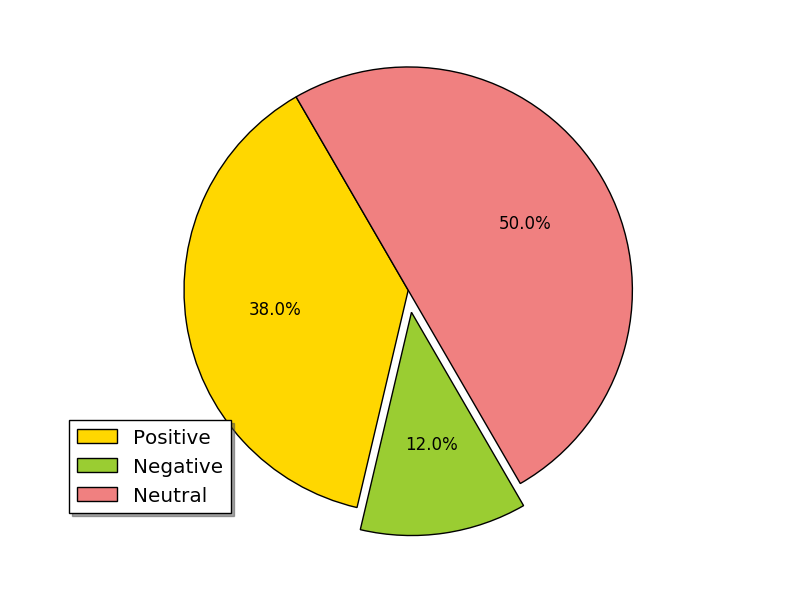
\includegraphics[scale=0.36]{Pie_TextBLOB.png}
\end{center}
\centering
\caption{Sentiment Scores using TextBLOB}
\end{figure} 
While reproducing the usecase, we have intensionally used NLTK (Refer Fig 3) replacing TextBLOB (Refer Fig 2), for the same set of tweets. Positive, Negative and Neutral sentiment percentages using TextBLOB are \emph{38.0\%}, \emph{12.0\%} and \emph{50.0\%} respectively. Whereas NLTK computes \emph{18.0\%}, \emph{17.0\%} and \emph{65.0\%} as Positive, Negative and Neutral percentages respectively.  
In this case, $Y$ != $Y'$ when trying to mock the case  \{$P$, $X$, $D'$\} where $D$ refers TextBLOB and  $D'$ refers NLTK respectively.

\begin{figure}[H]
\begin{center}
            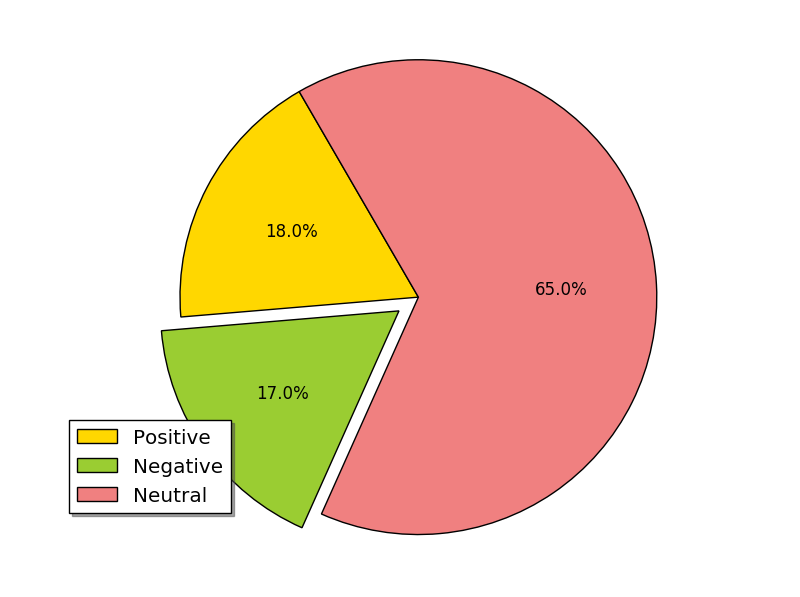
\includegraphics[scale=0.33]{Pie_NLTK.png}
\end{center}
\centering
\caption{Sentiment Scores using NLTK}
\end{figure} 
We have observed a striking difference in the results when using different software dependencies keeping the Program and Input unchanged. We viewed TextBLOB and NLTK as a blackbox and recorded the provenance of the two scripts without bothering about the algorithm design of TextBLOB and NLTK.  Motivated by the different results from related computations, we have analysed the provenance data collected by YesWorkflow and NoWorkflow.  \enquote{YesWorkflow} and \enquote{noWorkflow} are the tools that captures the provenance of independent scripts. ‘YesWorkflow’\textsuperscript{\cite{McPhillips2015}} extracts the latent information from scripts, exports, visualize in graph form. Given a script, YesWorkflow generates the workflow based on user annotations which generally captures prospective provenance.
\enquote{noWorkflow}\textsuperscript{\cite{Pimentel2015}} (not only Workflow) system uses Python runtime profiling functions to generate provenance traces that reflect the processing history of the script. ‘noWorkflow’ captures three types of provenance - definition, deployment, and execution provenance. 
\subsection{YesWorkflow}
YesWorkflow is one of the approach to capture prospective provenance from scripts. It helps to interpret the user annotations and visualise the graph that shows the computational steps and data flow in the script.We used YesWorkflow to visualize the graph to extract the API dependency (‘TextBLOB’ or ‘NLTK’) and retrieved two graphs showing the dependency. Furthermore, it is also possible to visualize the upstream and downstream of a specific data product. In addition to the visualization, YesWorkflow facilitates querying the workflow steps. The user annotations in the script play key role here. This provides very basic prospective provenance which is inadequate for analysing difference between the two execution results.
\subsection{NoWorkflow}
Noworkflow is another tool that captures the retrospective provenance automatically. It does not require user annotations for recording provenance. NoWorkflow defines one execution of the experiment as ‘Trial’. Here, the execution of Sentiment analysis with TextBLOB is referred as Trial 1 whereas  the execution with NLTK referred as Trial 2.
\enquote{NoWorkflow} has a command called \enquote{Diff} which yields a difference graph between 2 executions. 

For more details, please visit \url{http://eprint.ncl.ac.uk/file_store/production/234967/D959C504-4859-434A-A59A-8B7DC13AC4BD.pdf}

\section{Chapter II}
The main contribution for the chapter II is the \enquote{Why-Diff} algorithm which is able to compare two workflows by \enquote{forward} and \enquote{backward} traversals. 

\begin{enumerate} \label{data}
\item[1.] Forward traversal is to find the divergent data nodes that resulted due to change in the artefacts that the researcher voluntarily made self. This aims to traverse the provenance graph of computational steps with experimental input as a starting point. In this case, we aim to provide evidence that the changes have achieved the observed impact.
\item[2.] Backward traversal is to find the divergent activity nodes that caused the change that the Researcher unaware of self.This aims to traverse the provenance graph backwards to trace the causes that explain the difference with experimental output as a starting point. By doing so, we aim to find the likely causes for the observed differences in the outputs.
\end{enumerate}
eScience Central, shortly called as \enquote{e-SC}, is a Workflow Management System which provides Software and Platform as a Service to scientists to create, edit, run and share Workflows in the cloud \textsuperscript{\cite{Hiden2012}}. It captures very rich provenance information including data access and Workflow executions. The usage of these provenance details varies from one to another. Some might be interested who created the workflow, who downloaded it, who the data has been shared with. In our perspective, we are looking for what are the workflow inputs, outputs, services and intermediate results.  

\subsection{Technologies and standards used}
\begin{figure}[H]
  \centering
  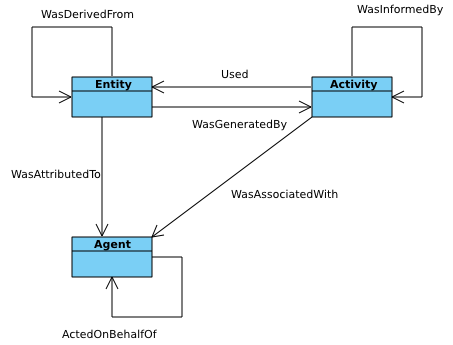
\includegraphics[scale=0.73]{ProvDM.png}
  \caption{PROV Core Structures}
  \label{fig:PROV-DM: The PROV Data Model}
\end{figure}

\setlength{\arrayrulewidth}{0.8mm}
\setlength{\tabcolsep}{15pt}
\renewcommand{\arraystretch}{1.3}
\begin{table}[H]
\caption{Provenance Terms Mapping}
\label{my-label}
\begin{tabular}{ |p{1.90cm}|p{1.90cm}|p{1.90cm}|  }
\hline
e-SC Format & PROV Format &  Neo4j\\
\hline
Document & Entity & Node\\
Execution & Activity  & Node\\
used & used & Relationship\\
wasGeneratedBy & wasGeneratedBy & Relationship\\
\hline
\end{tabular}
\end{table}

\begin{figure*}[!htp]
  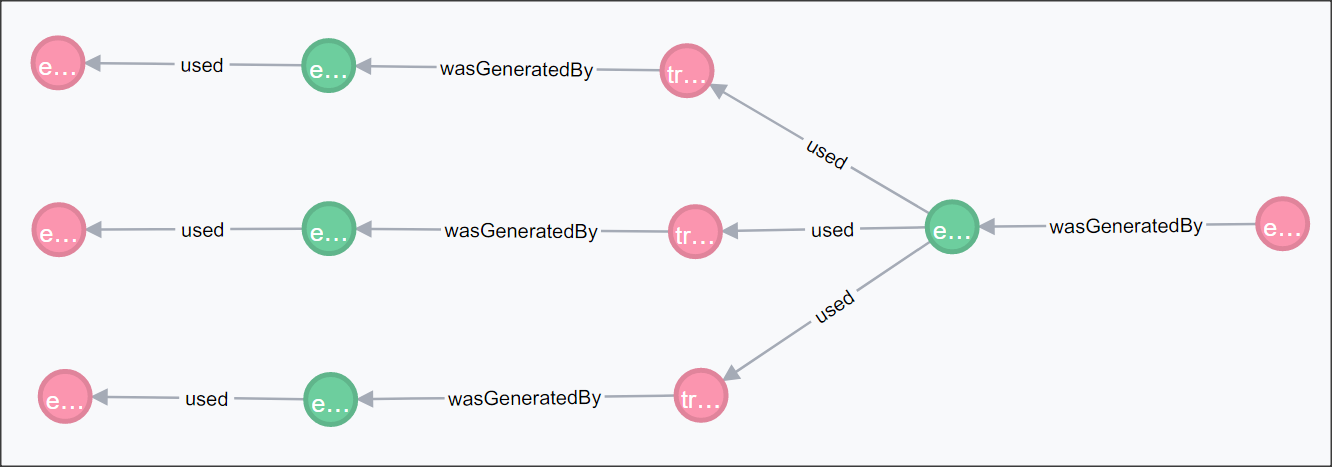
\includegraphics[width=18cm,height=5.5cm]{Simple_Workflow.png}
  \caption{Neo4j visualization of Sample Workflow}
\label{fig:Simple Workflow}
\end{figure*}

Each input and output files are given identities and file labels. Additionally each service in a particular workflow are given identities as well as service's configuration are updated. Intermediate files are given hash-values. Having all these piece of data together, we can able to answer why the results of 2 Workflows different and what is the result if a service version is
changed say for example from $version1$ to $version2$.
In order to verfiy the results of reproduced workflow in accordance with original workflow, an inbuilt differencing system like \enquote{Why-Diff} is mandatory.  The Workflow execution provenance of e-SC stick to the PROV-DM format. We have collected the Workflow execution provenance of eScience Central and have visualised in form of Neo4j nodes and relationships.

\subsection{Provenance Model}
W3C PROV \textsuperscript{\cite{ProvDM}} defines a data model and a set of constraints. It represents provenance as a Directed Acyclic Graph. Vertices in the PROV model represents entities, activities or agents. As scientists use different Workflow Management Systems, the provenance generated by such systems are in different format. To address this problem, an integration model ProvONE \textsuperscript{\cite{oliveira2016}} which takes in the provenance traces of heterogeneous workflow systems and generated integrated provenance database as Prolog facts. To have a common understanding of capabilities of different provenance systems, a data model was crafted by the authors and released as PROV-DM. PROV-DM is conceptual data model that has following nodes and relationships. Nodes are identified by prov:Activity, proc:Entity, prov:Agent, and relationship types are identified by prov:used, prov:wasInformedBy, prov:wasAssociatedWith, prov:wasGeneratedBy, prov:wasAttributedTo, prov:wasDerivedFrom, prov:actedOnBehalfOf. \enquote{Entity} refers to Physical, digital, conceptual, or other kind of thing with some fixed aspects; entities may be real
or imaginary. An \enquote{Activity} is something that occurs over a period of time and acts upon or with entities. An \enquote{Agent} is something that bears some form of responsibility for an activity taking place, for the existence of an entity, or for another agent’s activity. \enquote{wasGeneratedBy} refers to relationship between entity and activity, saying the entity was generated by the
activity. The relationship \enquote{used} infers that an entity is used by the activity and \enquote{wasDerivedFrom} refers to an entity being derived from another entity. As name indicates,\enquote{wasAssociatedWith} refers to an activity being associated to an Agent. \enquote{wasInformedBy} infers an activity being informed by another activity about an entity. \enquote{actedOnBehalfOf} refers to an agent acting on behalf of another agent. \enquote{wasAttributedTo} refers to an entity being attributed to an agent. 

\subsection{Why Neo4j?}
In our project, we have taken advantage of the most popular graph database \enquote{Neo4j}.  The graph database Neo4j is used in majority of fields like Chemistry, social network, semantic web, etc as it enables querying in simple manner in comparison to typical relational database. \newline

In e-SC, the number of available Workflows, services and datasets is constantly increasing. In order to accommodate large voluminous data, the optimal choice would be graph database.
Relational database could not handle these datasets as that needs complex join queries. To traverse the high-interconnected Workflow graphs which is  combination of entities and activities, Neo4j could be the advantageous. We have analysed Workflow execution provenance of  e-SC by exploiting PROV-DM and Neo4j. The Table I represents the provenance terms in e-SC, PROV-DM and Neo4j formats. In the figure 5, all the pink nodes are \enquote{entities} whereas green nodes are activities. The flow of graph starts from left to right. Relationships are identified as \enquote{used}  and \enquote{wasGeneratedBy}.

\subsection{WhyDiff}
\begin{algorithm}[!htbp]
  \caption{Forward Traversal}
	\label{}
\KwIn{Invocation1\_Id}
\KwIn{Invocation2\_Id}
\KwOut{$\Delta$ Graph}
\SetKwProg{Fn}{Function}{}{}
\SetKwRepeat{Do}{do}{while}%
$ Compare$ $the$ $list$ $of$ $first$ $Entities$ $in$ $both$ $graphs$\;
$first\_hop = true$\;
\Do{$firstActivityNewList \neq Empty$  \&\& $secondActivityNewList \neq Empty$}{
\eIf{$first\_hop == true$}
 {
$List<Activity> Activity1List \gets findFirstActivityList(Invocation1\_Id)$\;
$List<Activity> Activity2List \gets findFirstActivityList(Invocation2\_Id)$\;
 }
{
$List<Activity> Activity1List  \gets firstActivityNewList$\;
$List<Activity> Activity2List \gets secondActivityNewList$\;
$ClearfirstActivityNewList$ \& $secondActivityNewList$\;
}
\ForEach {$(A1,A2) \in  zip(Activity1List, Activity2List)$}{
$List<Entity> Entity1List \gets getWasGeneratedBy(A1)$\;
$List<Entity> Entity2List \gets getWasGeneratedBy(A2)$\;
\ForEach {$(E1,E2) \in  zip(Entity1List, Entity2List)$}{
$\Delta Graph \gets Compare(E1,E2)$; \newline
$List<Activity> returnedActivityList1 \gets getUsed(E1)$\;
$List<Activity> returnedActivityList2 \gets getUsed(E2)$\;
\ForEach {$(A1,A2) \in  zip(returnedActivityList1, returnedActivityList2)$}{
$Add$ $A1$ $to$ $firstActivityNewList$\;
$Add$ $A2$ $to$ $secondActivityNewList$\;
}
}
}
}
$ Compare$ $the$ $list$ $of$ $last$ $Entities$ $in$ $both$ $graphs$\;
\Fn{Compare (E1, E2)}{ 
\If{$E1.fileLabel \neq E2.fileLabel$}
{
$\Delta Graph \gets (E1, E2) $\; 
}
\Return $\Delta Graph$
}
\Fn{findFirstActivityList (InvocationId)}{
$List$ $all$ $activityNodes$ $WHERE$ $activity-[USED]-entity$ $WHERE$ $NOT$ $entity-[WASGENERATEDBY]-any\_activity$ $AND$ $activity.id$ $CONTAINS$ $InvocationId$\;
\Return activityNodes
}
\end{algorithm}

Why-Diff focuses on the execution provenance of the Workflows rather than the provenance of the Workflows itself. This relies on the execution provenance that are collected by E-Science Central WfMS. As mentioned in our previous work \textsuperscript{\cite{thavasimani2016}}, the accuracy of the Why-Diff analysis is proportional to the amount of provenance details of the two Workflows.

The project ‘Why-Diff’ consider 4 possible cases which resulted in output of reproduced computation different from output of original computation.
\begin{enumerate} \label{data}
\item[1.] \{$W$,$ X$, $D'$\} - Changing Dependency keeping Workflow, input unchanged.
\item[2.] \{$W$, $X'$, $D$\} - Changing Input keeping Workflow, Dependency unchanged.
\item[3.] \{$W'$, $X$, $D$\} - Changing Workflow keeping Dependency, input unchanged.
\item[4.] \{$W'$, $X'$, $D'$\} - All artefacts changed.
\end{enumerate}

We consider the difference in the Workflow results may be intentional or unintentional. Intentional changes are something that the experimenter is making himself/herself whereas unintentional changes are the changes that is made without the knowledge of the experimenter (For example updated external dependencies or external data sources which is not actually in control of the experimenter). In our previous work \textsuperscript{\cite{thavasimani2016}}, We have considered above cases and proved that there is possibility of the output difference when there is no change in Inputs $X$ and Program $P$ changing the Dependency $D$ to $D'$, mocking the scenario \{$P$, $X$, $D'$\}. The same applies to Workflows as well except the fact the Program $P$ represents orchestration of Program statements where Workflow $W$ represents orchestration of services. While tracking provenance of independent scripts, it is essential to keep track of each data product produced or consumed out of a particular program statement. In contrast to the scripts, workflows express the computations as service-level components. It considers each computational block as a service, which makes it feasible to compare two workflows based on the service version. It is more convenient to visually relate the Workflow steps which consumes data and produce data in the form of graph. At this early stage of our investigation, we make the simplifying assumption that the provenance graphs for the two executions are isomorphic, and only focus on detecting differences in properties of corresponding nodes. We use the retrospective provenance of the Workflow but not the abstract provenance of the Workflow. The Workflows to be compared are structurally similar (i.e. isomorphic). This is the simplest possible scenario where the topologies of the two graphs are identical, and only the properties on the nodes differ from one graph to another. 

\subsubsection{Forward Traversal}
 Algorithm I is designed to move forward the provenance graph to detect diverging entity nodes because of an intentional change introduced by the experimenter himself. If the changes are introduced intentionally, then the experimenter would like to know the effect (data difference that is resulted) of the change.  Hence he/she   forward traverse the graph to identify the data nodes that are not similar in both  the Workflow graphs. We consider this as \enquote{effect-analysis}. In the algorithm, we have used symbols $E1$, $E2$, $A1$, $A2$ to refer entity node for first invocation , entity node for second invocation, activity node for first invocation, activity node for second invocation respectively. The start nodes of the traversal are picked by listing the activities which have used an entity which is not generated by any other activity. As the traversal proceeds, for each activity, the generated entities are compared. The traversal continues till generated entities have not been used by any further activity. The traversal compares the file label (or hash value) initially. In eScience central WfMS, the end nodes are attached with file label property which is used to find the physical file name. The intermediate (we refer as transient) files possess the \enquote{hash value} property which is the unique identity of the transient data. All the diverging entities are added to the $\Delta$ Graph. The zip function in the algorithm ensures that the nodes from graph\textsubscript{1} are compared with the corresponding nodes in graph\textsubscript{2}. 
\subsubsection{Backward Traversal}
\begin{algorithm}[!htbp]
  \caption{Backward Traversal}
	\label{}
\KwIn{Invocation1\_Id}
\KwIn{Invocation2\_Id}
\KwOut{$\Delta$ Graph}
\SetKwProg{Fn}{Function}{}{}
\SetKwRepeat{Do}{do}{while}%
$first\_hop = true$\;
\Do{$firstActivityNewList \neq Empty$  \&\& $secondActivityNewList \neq Empty$}{
\eIf{$first\_hop == true$}
 {
$List<Activity> Activity1List \gets findLastActivityList(Invocation1\_Id)$\;
$List<Activity> Activity2List \gets findLasttActivityList(Invocation2\_Id)$\;
 }
{
$List<Activity> Activity1List  \gets firstActivityNewList$\;
$List<Activity> Activity2List \gets secondActivityNewList$\;
$ClearfirstActivityNewList$ \& $secondActivityNewList$\;
}
\ForEach {$(A1,A2) \in  zip(Activity1List, Activity2List)$}{
$\Delta Graph \gets Compare(A1, A2)$; \newline
$List<Entity> Entity1List \gets getUsed(A1)$\;
$List<Entity> Entity2List \gets getUsed(A2)$\;
\ForEach {$(E1,E2) \in  zip(Entity1List, Entity2List)$}{
$List<Activity> returnedActivityList1 \gets getWasGeneratedBy(E1)$\;
$List<Activity>returnedActivityList2 \gets getWasGeneratedBy(E2)$\;
\ForEach {$(A1,A2) \in  zip(returnedActivityList1, returnedActivityList2)$}{
$\Delta Graph \gets Compare(A1, A2)$; \newline
$Add$ $A1$ $to$ $firstActivityNewList$\;
$Add$ $A2$ $to$ $secondActivityNewList$\;
}
}
}
}
\Fn{Compare (A1, A2)}{
\If{$A1.configuration \neq A2.configuration$}
{
$\Delta Graph \gets (A1, A2) $\; 
}
\Return $\Delta Graph$
}
\Fn{findLastActivityList(InvocationId)}{
$List$ $all$ $activityNodes$ $WHERE$ $entity-[WASGENERATEDBY]- activity$ $WHERE$ $NOT$ $any\_activity-[USED]-entity$ $AND$ $activity.id$ $CONTAINS$ $InvocationId$\;
\Return activityNodes
}
\end{algorithm}
Algorithm II is designed to move backward the provenance graph to detect diverging activity nodes because of an unintentional change which the experimenter does not know. If the changes are unintentional then the experimenter would like to know the cause (activity node that caused the difference). And so he/she backward traverse the graph to identify the activity nodes that are not similar in both the Workflow graphs. This can be termed as \enquote{cause-analysis}. In the algorithm, we have used symbols $E1$, $E2$, $A1$, $A2$ to refer entity node for first invocation , entity node for second invocation, activity node for first invocation, activity node for second invocation respectively. The start nodes of the traversal are picked by listing the activities which have \enquote{generated} an entity which is further not \enquote{used} by any other activity. As the traversal proceeds, each activity configuration are compared and for each activity the \enquote{used} entities are identified. The traversal continues till \enquote{used} entities have not been generated by any further activity. In eScience central WfMS, each activity are associated with configuration property, which captures good provenance of which the interesting ones are the file labels it has used/ generated, library used, the conditions it has used, source file used, block name and version. These metadata will help us comparing one activity node to another and all the diverging activities are added to the $\Delta$ Graph. The zip function in the algorithm ensures that the nodes from graph\textsubscript{1} are compared with the corresponding nodes in graph\textsubscript{2}. 

\section{Chapter III}
The main contribution is  a tool \enquote{Why-Diff}  which is able to analyse the differences between any two workflow runs by exploiting the execution provenance associated with the workflow.  
\begin{itemize}
\item[1.] Possible Variations between Original and Reproduced Computations: As we already introduced the notations {$W$, $X$, $D$} as Workflow, Input and Dependencies and variation to these could affect the final result. Variation to the input i.e. $X$ could be $X'$ and $D$ could be $D'$ which can be introduced in reproduced workflows by changing the input entities in the workflow. However variation to the workflow i.e. $W$ to $W'$ actually mean a new task has been added to the workflow, an existing task is deleted from the workflow or updation of existing task. To mitigate this, we come up with real-time cases of workflow evolution.
\begin{itemize}
\item[a.] Addition of new activities.
\item[b.] Deletion of existing activities. 
\item[c.] Updated version of existing activities.
\end{itemize} 
For example consider an Workflow W which consists of workflow blocks [$w1$, $w2$, $w3$, $w4$, $w5$]. In the reproduced workflow W', there could be an insertion of $w6$ i.e [$w1$, $w2$, $w3$, $w4$, $w5$, $w6$], or deletion of $w2$ i.e. [$w1$, $w3$, $w4$, $w5$] or updating an existing activity $w4$ i.e. [$w1$, $w2$, $w3$, $w4'$, $w5$] or combination of all these. Here the addition and deletion of workflow blocks give raise to the non-isomorphic cases where a workflow node is not present in the other graph.
\item[2.] Why-Diff - an extension of our previous algorithm \cite{Priyaa} is to find the divergent activity and data nodes that resulted to support non-isomorpic cases.  This  aims  to traverse the provenance graph of workflow to trace the causes that explain the difference. By doing so, we aim to find the causes for the observed differences in the outputs. 
\item[3.] Content-based differencing between entities of the comparing workflows.
\item[4.] $\Delta$ graph - a GraphViz implementation of graph visualisation, comprising of matching nodes from comparing workflow, and highlighting the unmatching nodes with subgraph.
\end{itemize} 

\subsection{Technical Approach}
Figue 1(a) and 1(b) represents the insertion/deletion of activity respectively. The model that we exhibit here follows PROV-DM \cite{ProvDM}, where all data produced/consumed is an \enquote{entity} (oval-shaped nodes) and the workflow blocks which uses/generates an entity is an \enquote{activity} (box-shaped nodes). The \enquote{used} relationships are represented in blue arrows and the \enquote{wasGeneratedBy} relationships are represented in brown arrows. The orange-dashed lines link the matching/corresponding nodes. By terming it as corresponding activity, we clarify that the activity node in first graph may or may not be equal as the activity node in the second graph, however, they both are similar.  And green dashed line links \enquote{sync} nodes which is the first matching node after the divergence.  
\begin{enumerate} \label{data}
\item[1.] Activity Insertion:
This refers to the insertion of a single workflow block to the reproduced workflow. Fig:1.a represents the sample activity insertion where $E3$ is generated because of the insertion of new Activity $A2$. 
\item[2.] Activity Deletion:
This refers to the deletion of a single workflow block to the reproduced workflow. Fig:2.b represents that an activity $A2$ is removed in second workflow and hence there is no existence of $E3$.
\item[2.] Activity Update:
This refers to the update of a single workflow block to the reproduced workflow. Fig:3.b represents that an activity $A3$ is replaced in second workflow with $E3'$.
\begin{figure*}
\centering
\begin{subfigure}{.33\textwidth}
  \centering
  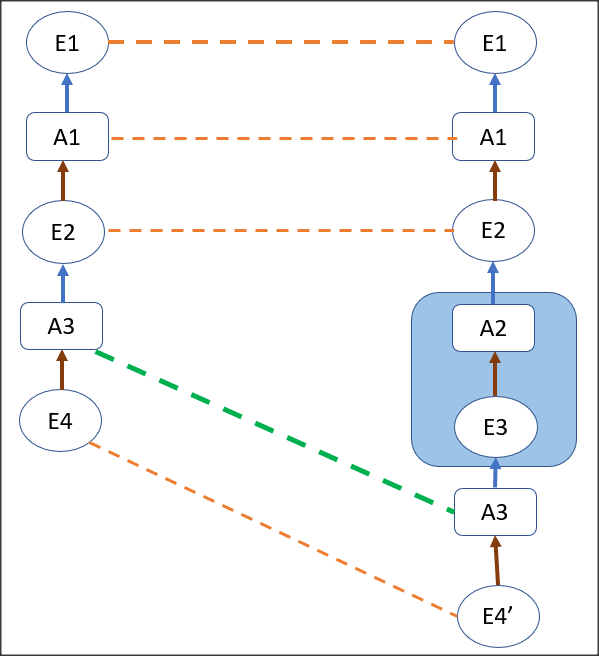
\includegraphics[width=5.5cm,height=7cm]{ActivityInsertion.png}
  \caption{Activity Insertion (Non-isomorphic)}
\label{fig: Activity Insertion}
\end{subfigure}%
\begin{subfigure}{.33\textwidth}
  \centering
   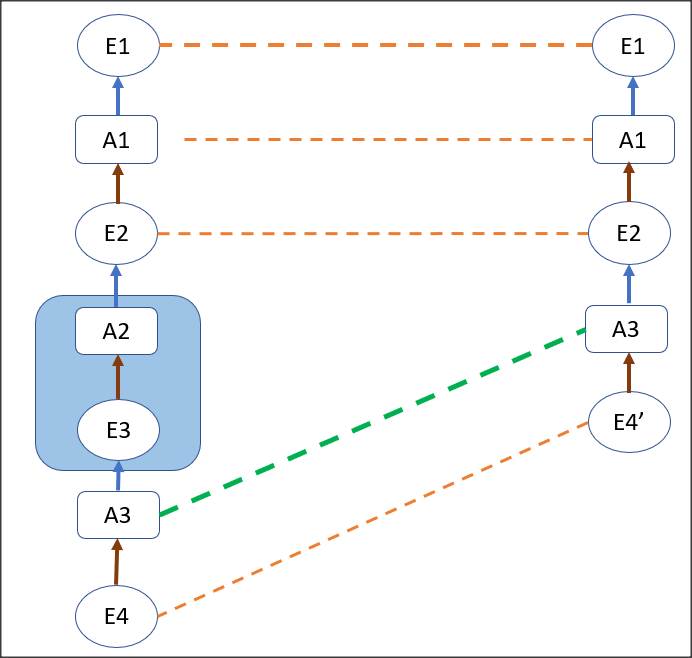
\includegraphics[width=5.5cm,height=7cm]{ActivityDeletion.png}
  \caption{Activity Deletion (Non-isomorphic)}
\label{fig: Activity Deletion}
\end{subfigure}
\begin{subfigure}{.33\textwidth}
  \centering
  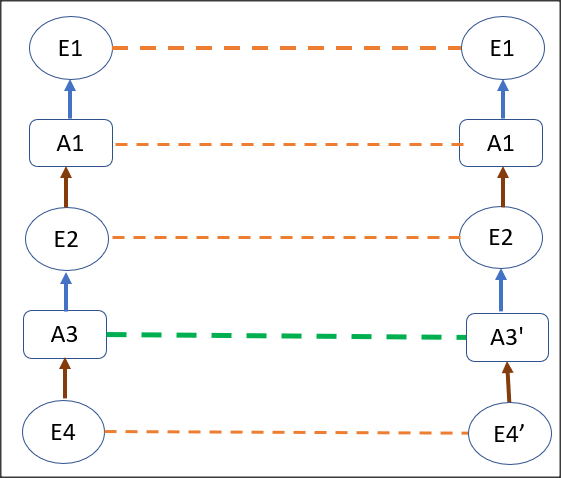
\includegraphics[width=5.5cm,height=7cm]{ActivityUpdate.png}
  \caption{Activity Update (Isomorphic)}
\label{fig: Activity Update}
\end{subfigure}%
\label{fig:test}
\caption{Activity Insertion, Deletion and Update}
\end{figure*}
\end{enumerate}

\subsection{Why-Diff}
Why-Diff focuses on the execution provenance of the workflows rather than the provenance of the workflows itself. This relies on the execution provenance that is collected by WfMS. As mentioned in our previous work, the accuracy of the Why-Diff analysis depends on the amount of provenance details of the two workflows. The algorithm uses symbols  $E1$, $E2$, $A1$, $A2$ to refer entity node for 1\textsuperscript{st} invocation , entity node for 2\textsuperscript{nd} invocation, activity node for 1\textsuperscript{st} invocation, activity node for 1\textsuperscript{nd} invocation respectively. Algorithm is an extension of our previous work  \cite{Priyaa} which aims to find the divergent nodes so that know the cause for the different results. This compares two graphs which is not structurally similar. 

To start the traversal, the researcher should know the invocation ID of the two workflows that he/she wants to compare. The traversal starts by listing the activities which may have \enquote{used} an entity say $E$, which was \enquote{not generated} by any other activity. An activity can be uniquely identified using activity's id. Hence, the listed activites are zipped using \enquote{Zip} function which is to arrange the activities from first graph and second graph based on its ids.  This is to ensure the activities of the first graph is actually compared against the corresponding activity in the second graph. All the activities which is not zipped are added to the $List<unZippedNode>$ nodes. The `zipped' activites from first workflow are compared against the `zipped' activities of second workflow. The comparion is made to check whether the configuration of activity from first graph is equal to the configuration of activity from second graph. Some of the activity's configuration details that eScience Central Workflow Management Systems captures include AllowRetriesOnTimeOut, Condition used, DebugMode, DebugPort, DebugSuspended, Delimiters, EnforeInvocationTimeOut, ImportChunkSize, InvocationTimeout, Label, Name, Source, ProceedOnFail, TimeOutRetries. As the traversal proceeds, for each activity, the corresponding \enquote{generated} entities (zipped) are compared. Unzipped entities are added to the $List<unZippedNodes>$. The traversal stops when it reaches last node (i.e final output) in the workflow graph. If the activity node in the first workflow is not equal to the corresponding activity node in the second workflow, then those nodes are added to the list of diverging nodes which aids in representing difference graph. (i.e. $\Delta$ Graph).

\begin{tiny}
\begin{algorithm}
\scriptsize
 \caption{Why-Diff}
\KwIn{Invocation1\_Id,Invocation2\_Id}
\KwOut{$\Delta$ Graph}
\SetKwProg{Fn}{Function}{}{}
\SetKwRepeat{Do}{do}{while}%
% This is to hide end and get the last vertical line straight
\SetKwBlock{Begin}{Begin}{}
\SetAlgoLined
  \Begin{
 $ Compare$ $the$ $list$ $of$ $first$ \& $last$ $Entities$ $in$ $both$ $graphs$\;
$first\_hop = true$\;
\Do{$firstActivityNewList \neq Empty$ \&\& $secondActivityNewList \neq Empty$}{
\eIf{$first\_hop == true$}
 {
$List<Activity> Activity1List \gets findFirstActivityList(Invocation1\_Id)$\;
$List<Activity> Activity2List \gets findFirstActivityList(Invocation2\_Id)$\;
 }
{
$List<Activity> Activity1List  \gets firstActivityNewList$\;
$List<Activity> Activity2List \gets secondActivityNewList$\;
$ClearfirstActivityNewList$ \& $secondActivityNewList$\;
}
\ForEach {$(A1) \in firstActivityNewList$}{
\ForEach {$(A2) \in secondActivityNewList$}{
\If{$A1 \xi A2$}
{
$List<zippedNodes> \gets Add(A1, A2)$\; 
$List<divergingNodes> \gets Compare(A1, A2)$; 
}
{
$AddUnMatchedNodes(A1, A2)$;
}
$List<Entity> Entity1List \gets getWasGeneratedBy(A1)$\;
$List<Entity> Entity2List \gets getWasGeneratedBy(A2)$\;
\ForEach {$(E1) \in Entity1List$}{
\ForEach {$(E2) \in Entity2List$}{
$List<firstGraph> \gets Add(A1,\leftarrow,E1)$\; 
$List<secondGraph> \gets Add(A2,\leftarrow,E2)$\; 
\If{$E1 \xi E2$}
{
$List<zippedNodes> \gets Add(E1, E2)$;  
$List<divergingNodes> \gets Compare(E1,E2)$; 
}
{
$addUnMatchedNodes(E1, E2)$;
}
$List<Activity> returnedActivityList1 \gets getUsed(E1)$\;
$List<Activity> returnedActivityList2 \gets getUsed(E2)$\;
\ForEach {$(A1) \in returnedActivityList1$}{
\ForEach {$(A2) \in returnedActivityList2$}{
$List<firstGraph> \gets Add(E1,\leftarrow, A1)$\; 
$List<secondGraph> \gets Add(E2,\leftarrow, A2)$\; 
$List<firstActivityNewList> \gets Add(A1)$\;
$List<secondActivityNewList> \gets Add(A2)$\;
}
}
\If{$returnedActivityList1 \neq Empty \&\& returnedActivityList2 = Empty$}
{
$addExtraNodesFirstGraph(returnedActivityList1)$\;
}
\If{$returnedActivityList1 = Empty \&\& returnedActivityList2 \neq Empty$}
{
$addExtraNodesSecondGraph(returnedActivityList2)$\;
}
{
}
}
}
}
}
}
$resync()$\;
$constructDeltaGraph($List$<$firstGraph$>$$,$List$<$secondGraph$>$$
,$List$<$divergingNodes$>$$,$List$<$zippedNodes$>$$)$\;
\Fn{Compare (E1, E2)}{ 
\If{$E1 \neq E2$}
{
$List<divergingNodes>$ $<$$-$ $Add (E1, E2) $\; 
}
\Return $List<divergingNodes>$\;
}
 }
\end{algorithm}

\begin{algorithm}
\scriptsize
    \caption{Why-Diff}
\SetKwProg{Fn}{Function}{}{}
\SetKwRepeat{Do}{do}{while}%
\setcounter{AlgoLine}{12}
% This is to restore vline mode if you did not take the package as \usepackage[linesnumbered,ruled,vlined]{algorithm2e}
  \SetAlgoVlined
%This is to hide Begin keyword
\SetKwBlock{Begin}{}{end}
\Begin{
\Fn{resync()}{ 
\ForEach {$(Node1) \in List<firstExtra>$}{
\ForEach {$(Node2) \in List<secondExtra>$}{
\If{$Node1$ $is$ $a$ $Activity$ \&\& $Node2$ $is$ $a$ $Activity$}{
\If{$Node1 \xi Node2$}
{
$List<divergingNodes> \gets Compare(A1, A2)$;
}
}
{
\If{$Node1 \xi Node2$}
{
$List<divergingNodes> \gets Compare(E1, E2)$;
}
}
}
}
}
\Fn{addUnMatchedNodes(Node1, Node2)}{ 
$List<firstExtra> \gets Add(Node1)$;
$List<secondExtra> \gets Add(Node2)$;
$List<divergingNodes> \gets Add(Node1, ABSENT)$; 
$List<divergingNodes> \gets Add(ABSENT,Node2)$; 
}
\Fn{addExtraNodesFirstGraph(
returnedActivityList1)}{ 
\Do{$returnedActivityList1$ $has$ $Next$}
{
\ForEach {$(A1) \in returnedActivityList1$}{
$List<divergingNodes> \gets Add(Node1, ABSENT)$\; 
$List<firstExtra> \gets Add(Node1)$\;
$List<Entity> Entity1List \gets getWasGeneratedBy(A1)$\;
\ForEach {$(E1) \in Entity1List$}{
$List<divergingNodes> \gets Add(Node1, ABSENT)$\; 
$List<firstExtra> \gets Add(Node1)$\;
$List<Activity> returnedActivityList1 \gets getUsed(E1)$\;
}
}
}
}
\Fn{addExtraNodesSecondGraph(
returnedActivityList2)}{ 
\Do{$returnedActivityList1$ $has$ $Next$}
{
\ForEach {$(A1) \in returnedActivityList1$}{
$List<divergingNodes> \gets Add(ABSENT, Node2)$\; 
$List<secondExtra> \gets Add(Node2)$\;
$List<Entity> Entity1List \gets getWasGeneratedBy(A1)$\;
\ForEach {$(E1) \in Entity1List$}{
$List<secondExtra> \gets Add(Node2)$\;
$List<divergingNodes> \gets Add(ABSENT, Node1)$\; 
$List<Activity> returnedActivityList1 \gets getUsed(E1)$\;
}
}
}
}
\Fn{findFirstActivityList (InvocationId)}{
$List$ $all$ $activityNodes$ $WHERE$ $activity-[USED]-entity$ $WHERE$ $NOT$ $entity-[WASGENERATEDBY]-any\_activity$ $AND$ $activity.id$ $CONTAINS$ $InvocationId$\;
\Return activityNodes
}
\Fn{Compare (A1, A2)}{
\If{$A1.configuration \neq A2.configuration$}
{
$List<divergingNodes>$ $<$$-$ $Add (A1, A2) $\; 
}
\Return $List<divergingNodes>$\;
}
\Fn{constructDeltaGraph($List<firstGraph>$,$List<secondGraph>$,$List<divergingNodes>$,$List<zippedNodes>$)}
{
\ForEach{$row \in List<firstGraph>$}{
$\Delta Graph <- AddAll($row$)$\;
}
\ForEach{$row \in List<secondGraph>$}{
$\Delta Graph <- AddAll($row$)$\;
}
\ForEach{$Node1 \in List<zippedNodes> \&\& Node2 \in List<zippedNodes>$}{
$\Delta Graph <- Edit($Node1$,$Node1$\equiv$Node2$)$\;
$\Delta Graph <- Edit($Node2$,$Node1$\equiv$Node2$)$\;
}
\ForEach{$Node1 \notin List<zippedNodes> \parallel Node2 \notin List<zippedNodes>$}{
$SubGraph <- AddAll($Node1$, $Node2$)$\;
}
\ForEach{$roNodew \in List<divergingNodes>$}{
$\Delta Graph <- Edit(Node,peripheries="2",style="filled", fillcolor="mediumspringgreen", color="orangered")$\;
}
\Return $\Delta Graph$;
%$Highlight$ $unqual$ $nodes$ $with$ $red$ $borders$\;
%$Cluster$ $and$ $highlight$ $unzipped$ $nodes$ $in$ $subgraph$\;
} 
  }
\end{algorithm}
\end{tiny}

\setlength{\textfloatsep}{5pt}
In eScience central WfMS, the entity nodes are attached to file label property which is used to find the physical file name. So, we compare the contents of these nodes. The intermediate (we refer as transient) files possess the \enquote{hash value} property which helps to identify unique transient data. For these intermediate nodes, we comapre hash-values. If the file label or the hash value of entity node in the first workflow is not equal to the file label or hash value of its corresponding entity node in the second workflow, then those nodes are added to the list of diverging nodes which aids in representing difference graph. (i.e. $\Delta$ Graph). To handle non-isomorphic cases, all the extra nodes are added to the $List<divergingNodes>$. Further, we keep track of all unzipped nodes during the traversal and try to resync each unzipped node with the every node in the $List<divergingNodes>$ to find the sync node. The sync nodes are compared and the  diverging node list is updated accordingly. We use the $List<divergingNodes>$ and $List<zippedNodes>$ to construct the delta graph. 
\subsection{Visual Representation of Delta Graph with GraphViz}
To visually represent the delta graph, we make use of GraphViz. GraphViz is a open-source software, which facilitates to draw graphs specified in DOT\cite{GraphViz}. All the entities are represented in pink-oval shaped nodes and all the activities are represented in green-box shaped nodes. All the entity names of first and second graphs are represented by `$e$' with subscript 1 and 2 respectively, followed by the node number. All the activity names of first and second graphs are represented by `$a$' with subscript 1 and 2 respectively, followed by the node number. For example, `$e\textsubscript{1}2$' refers to the  2\textsuperscript{nd} entity of first graph and `$a\textsubscript{2}3$' refers to the 3\textsuperscript{rd} activity of second graph. 
If the entity/activity from 1\textsuperscript{st} graph is matched/zipped with node in 2\textsuperscript{nd} graph, it is represented with `$\equiv$' equivalent symbol. For example, `$e\textsubscript{1}2$$\equiv$$e\textsubscript{2}2$' indicates 2\textsuperscript{nd} entity from 1\textsuperscript{st} graph is equivalent to 2\textsuperscript{nd} entity from  2\textsuperscript{nd} graph.
Subgraphs specify semantic information about graph components. GraphViz provides facility to group certain nodes and edges in the form of subgraph which we made use of highlighting the unmatched/unzipped nodes as well as unmatched edges. To highlight the unequal nodes, the node attribute \enquote{peripheries} is set to 2 so that to have two borders for a node.


\section{Research Outputs}
\begin{figure*}
\centering
\begin{subfigure}{.75\textwidth}
  \centering
  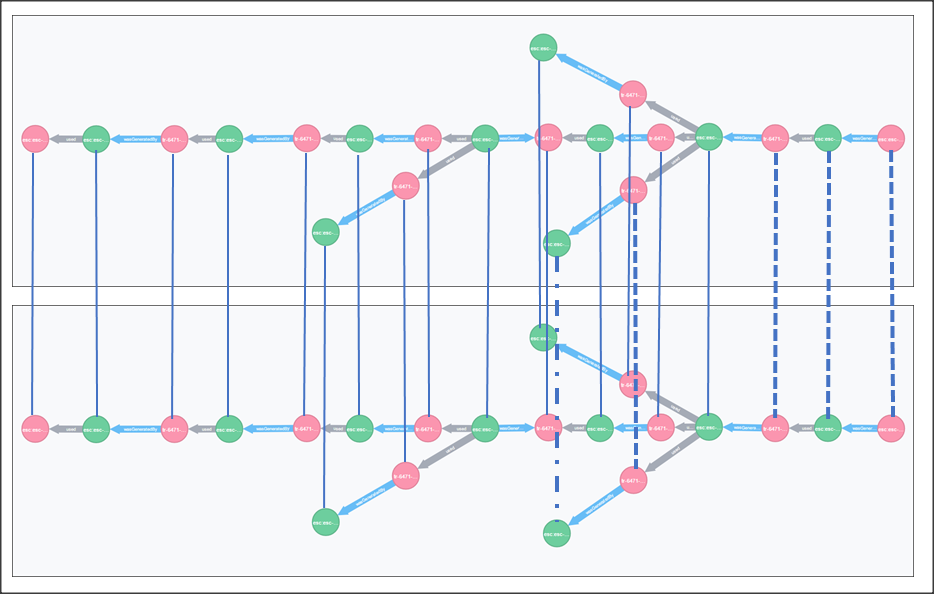
\includegraphics[width=13cm,height=7cm]{Difference_Graph.png}
  \caption{Difference Graph of Freebayes}
\label{fig:Difference Graph of Freebayes}
\end{subfigure}%
\begin{subfigure}{.25\textwidth}
   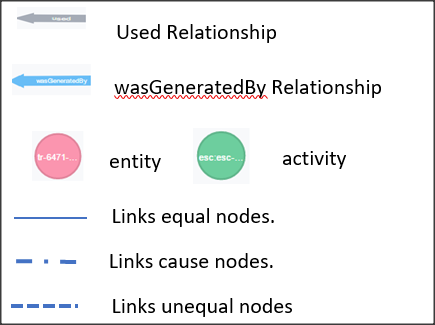
\includegraphics[width=5cm,height=4cm]{Graph_Symbols.png}
  \caption{Notations}
\label{fig:Notations}
\end{subfigure}
\label{fig:test}
\caption{Comparison graph of Freebayes and notations used}
\end{figure*}
\subsection{Usecase - Freebayes Variant Calling}
The use case we worked with was the Freebayes variant calling workflow. It processes aligned patient sequence files (in the BAM format) in the search for variants from the reference genome. The main source of change in this workflow is the version of Freebayes tool used (https://github.com/ekg/freebayes). Over the last three years the author has released about 15 versions of the program and so an important question is whether and to what extent these changes affect the output. 
\subsubsection{Evaluation of Freebayes Workflow}
In fig 6, we have visualised the graphs of the two Freebayes invocations of which the top graph represents invovation $6471$ whereas the bottom graph represents invocation $5463$. The difference between the invocations are such that $6471$ has used Freebayes library of version $Freebayes-1.0.2$ whereas $5463$ has used $Freebayes-0.9.10$. To spot similar, dissimilar and cause nodes, we have used three types of lines. The straight line refers the two linked nodes are equal. \enquote{Dashed} lines link the nodes that are not equal. \enquote{Dashed dot} lines link the nodes that actually caused the difference. 

We have tested the algorithm with another usecase \enquote{Simple Variant Interpretation (SVI)}, which was implemented as part of Re-Comp  project (recomp.org.uk). SVI is a workflow which takes advantage of two external data sources OMIM GeneMap and NCBI ClinVar to provide interpretation of human variants to facilitate clinical diagnosis of genetic diseases say for example, Alzheimer's disease. We have observed above stated “Why-Diff” scenario in SVI Workflow. For more results on SVI, please visit  \url{https://github.com/Priyaa140624191/Why-Diff/blob/master/WhyDiffAlgorithm/SVI%20Results.pdf}

\subsection{Workflow Comparison supporting Non-Isomorphic Cases}
The figure Fig.8(a) shows the comparison between two workflows, in which activity `$a\textsubscript{2}1$' of first workflow has been inserted serially in reproduced computation. The resultant $\Delta$ Graph shows inserted nodes from the first workflow as subgraph. The `$a\textsubscript{1}2$$\equiv$$a\textsubscript{2}1$' refers `$a\textsubscript{1}2$' is equivalent to `$a\textsubscript{1}1$' but they are \enquote{unequal} as the node is highlighted with double-red borders. Hence, the cause for the difference in results (i.e. '$e\textsubscript{1}3$' is not equal to  `e\textsubscript{2}3') is because activity `$a\textsubscript{1}2$'  is replaced with activity `$a\textsubscript{2}1$' and the activity `$a\textsubscript{2}1$' is inserted. The figure Fig.8(b) shows activity deletion comparing same two workflows as Fig.8(a) by changing the order, thus the subgraph highlights the nodes deleted serially.
\begin{figure*}
\centering
\begin{subfigure}{.50\textwidth}
  \centering
  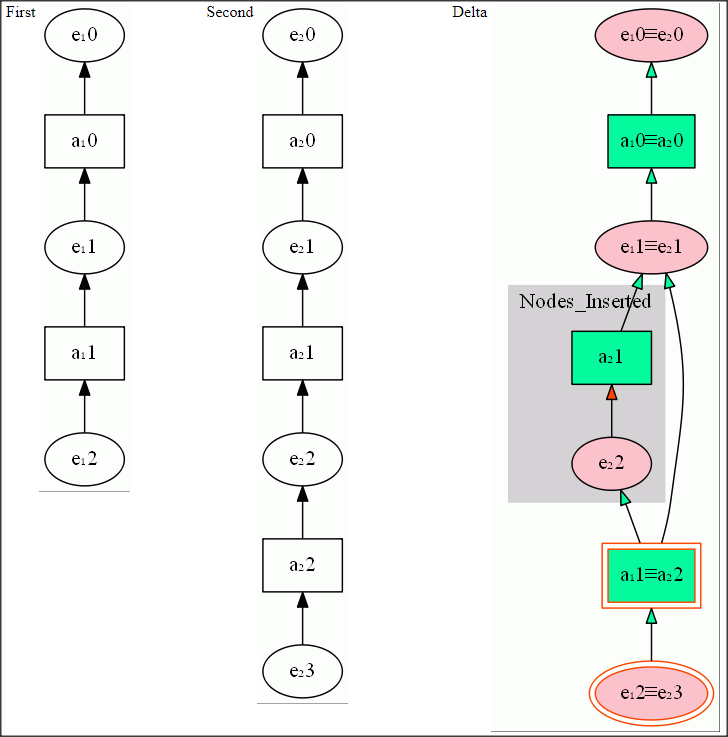
\includegraphics[width=6cm,height=6.5cm]{DeltaActivityInsertion.png}
  \caption{Activity Insertion}
  \label{fig:Activity Insertion}
\end{subfigure}%
\begin{subfigure}{.50\textwidth}
    \centering
  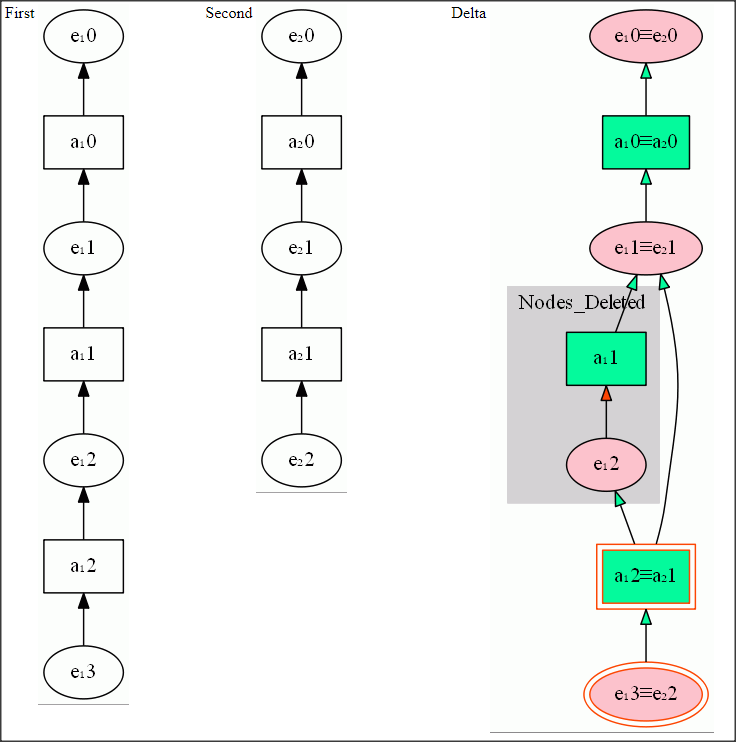
\includegraphics[width=6cm,height=6.5cm]{DeltaActivityDeletion.png}
  \caption{Activity Deletion}
  \label{fig:Activity Deletion}
\end{subfigure}
\label{fig:test}
\caption{Activity Insertion and Deletion}
\end{figure*}

The figure Fig.9(a) shows the comparison between two workflows, in which path comprising of activities `$a\textsubscript{2}2$' and `$a\textsubscript{2}4$' of first workflow has been inserted parallely in reproduced computation. The resultant $\Delta$ Graph shows inserted nodes from the first workflow as subgraph. The `$a\textsubscript{1}5$$\equiv$$a\textsubscript{2}3$' refers `$a\textsubscript{1}5$' is equivalent to `$a\textsubscript{1}3$' but they are \enquote{unequal} as the node is highlighted with double-red borders. Hence, the cause for the difference in results (i.e. `$e\textsubscript{1}6$' is not equal to  e\textsubscript{2}4') is because activity `$a\textsubscript{1}5$'  is replaced with activity `$a\textsubscript{2}3$' and the activities running parallely to existing activites`$a\textsubscript{2}2$' and `$a\textsubscript{2}4$' are removed. The figure Fig.9(b) shows path deletion comparing same two workflows as Fig.9(a) by changing the order, thus the subgraph highlights the path (comprising of nodes), deleted parallely.

\begin{figure*}
\centering
\begin{subfigure}{.50\textwidth}
  \centering
  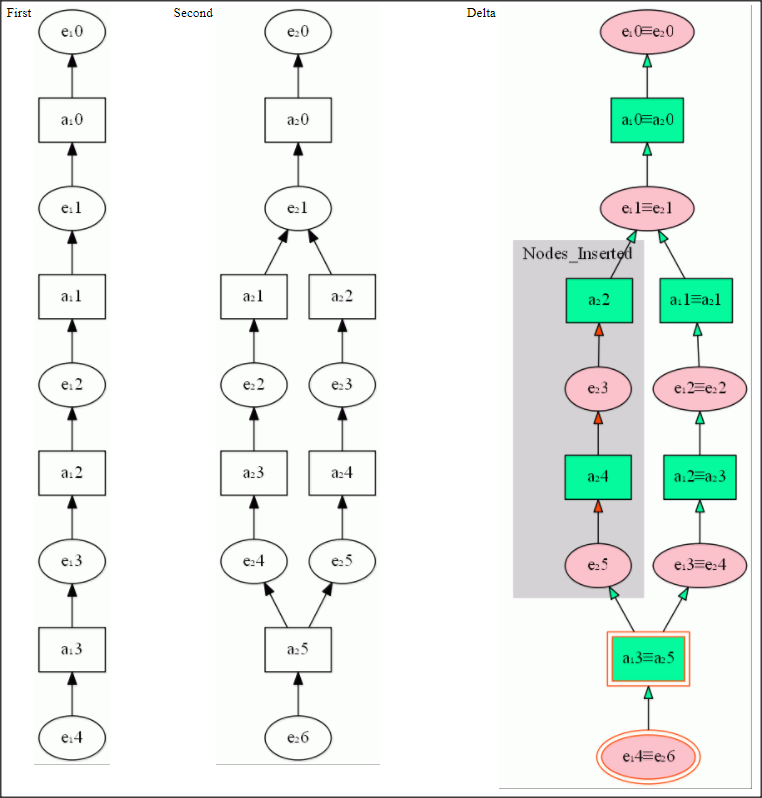
\includegraphics[width=6cm,height=7cm]{DeltaPathInsertion.png}
  \caption{Path Insertion}
  \label{fig:Path Insertion}
\end{subfigure}%
\begin{subfigure}{.50\textwidth}
    \centering
  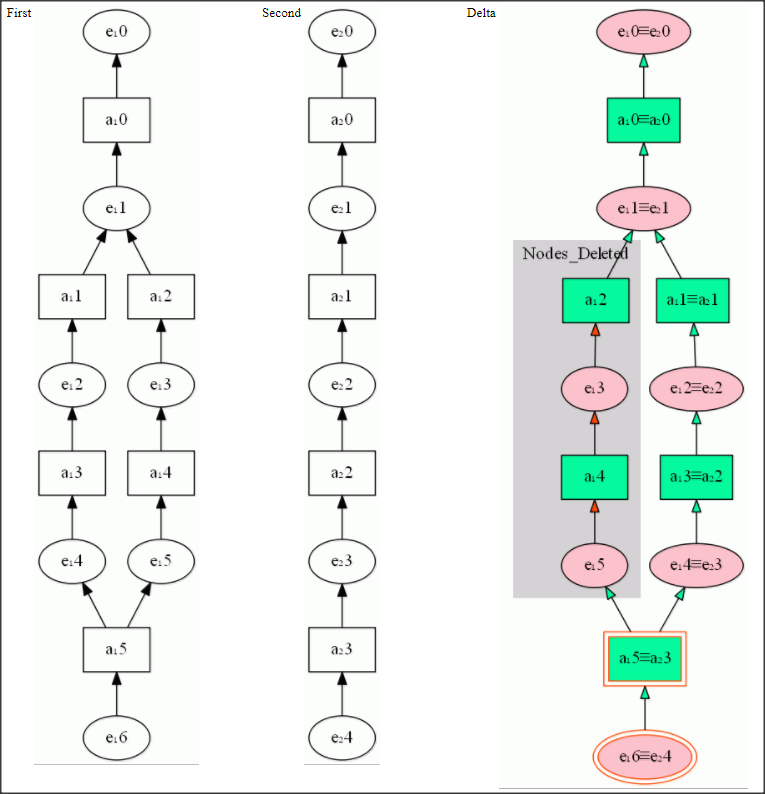
\includegraphics[width=6cm,height=7cm]{DeltaPathDeletion.png}
  \caption{Path Deletion}
  \label{fig:Path Deletion}
\end{subfigure}
\label{fig:test}
\caption{Path Insertion and Deletion}
\end{figure*}

The figure Fig.10(a) shows the comparison between two workflows, in which sub-workflow comprising of activities `$a\textsubscript{2}1$', `$a\textsubscript{2}2$', `$a\textsubscript{2}3$' and `$a\textsubscript{2}4$' of first workflow has been inserted in reproduced computation. This is complex scenario which is a combination of serial and parallel activity insertion. The resultant $\Delta$ Graph shows inserted nodes from the first workflow as subgraph. The `$a\textsubscript{1}5$$\equiv$$a\textsubscript{2}1$' refers `$a\textsubscript{1}5$' is equivalent to `$a\textsubscript{1}1$' but they are \enquote{unequal} as the node is highlighted with double-red borders. Hence, the cause for the difference in results (i.e. `$e\textsubscript{1}6$' is not equal to  `e\textsubscript{2}2') is because activity `$a\textsubscript{1}5$'  is replaced with activity `$a\textsubscript{2}1$' and the subworkflow (running serially to the existing activities) comparising of `$a\textsubscript{2}1$', `$a\textsubscript{2}2$', `$a\textsubscript{2}3$' and `$a\textsubscript{2}4$' is removed. The figure Fig.10(b) shows sub-workflow deletion comparing same two workflows as Fig.10(a) by changing the order, thus the subgraph highlights the sub-workflow (comprising of nodes) deleted.
\begin{figure*}
\centering
\begin{subfigure}{.50\textwidth}
  \centering
  \includegraphics[width=6cm,height=7cm]{DeltaSubGraphInsertion.png}
  \caption{Sub-Workflow Insertion}
  \label{fig:Sub-Workflow Insertion}
\end{subfigure}%
\begin{subfigure}{.50\textwidth}
    \centering
  \includegraphics[width=6cm,height=7cm]{DeltaSubGraphDeletion.png}
  \caption{Sub-Workflow Deletion}
  \label{fig:Sub-Workflow Deletion}
\end{subfigure}
\label{fig:test}
\caption{Sub-Workflow Insertion and Deletion}
\end{figure*}

\begin{figure}
  \centering
  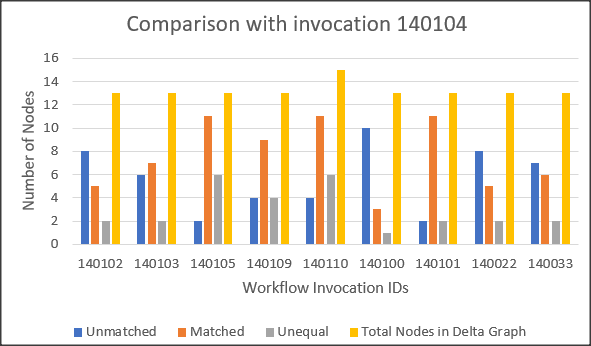
\includegraphics[scale=0.70]{WorkflowComparisons.png}
  \caption{Workflow Comparisons}
  \label{fig:Workflow Comparisons}
\end{figure}

\subsection{Evaluation}
We have tested `Why-Diff' with 10 similar workflows taking multiple variations into consideration, trying out all possible combinations changing artefacts {$W$, $X$, $Y$} to {$W'$, $X'$, $Y'$} as well as testing non-isomorphic cases (i.e. activity, path and subworkflow insertion/deletion). We have executed 45 comparisons among the 10 workflows. Figure.11 represents workflow comparisons of 140104 with 9 similar workflows (i.e. 140102, 140103, 140105, 140109, 140110, 140100, 140101, 140022, 140033). Number of matched, unmatched, unequal, total nodes in $\Delta$ Graph in each comparisons are represented in bar chart to figure out how the final results vary when inserting and/or deleting an activity while reproducing a workflow.
  
\bibliographystyle{IEEEtran}
\bibliography{MyCollection}
\end{document}





















































